\documentclass[12pt, a4paper, oneside]{ctexart}
\usepackage{amsmath, amsthm, amssymb, bm, color, graphicx, geometry, mathrsfs,extarrows, braket, booktabs, array, wrapfig, enumitem}
\usepackage[colorlinks,linkcolor=red,anchorcolor=blue,citecolor=blue,urlcolor=blue,menucolor=black]{hyperref}
%%%% 设置中文字体 %%%%
% fc-list -f "%{family}\n" :lang=zh >d:zhfont.txt 命令查看已有字体
\setCJKmainfont[
    BoldFont=方正黑体_GBK,  % 黑体
    ItalicFont=方正楷体_GBK,  % 楷体
    BoldItalicFont=方正粗楷简体,  % 粗楷体
    % Mapping = fullwidth-stop  % 将中文句号“.”全部转化为英文句号“.”
]{方正书宋简体}  % !!! 注意在Windows中运行请改为“方正书宋简体.ttf” !!!
%%%% 设置英文字体 %%%%
\setmainfont{Minion Pro}
\setsansfont{Calibri}
\setmonofont{Consolas}

%%%% 设置行间距与页边距 %%%%
\linespread{1.2}
%\geometry{left=2.54cm,right=2.54cm,top=3.18cm,bottom=3.18cm}
\geometry{left=1.84cm,right=1.84cm,top=2.18cm,bottom=2.18cm}

%%%% 图片相对路径 %%%%
\graphicspath{{figures/}} % 当前目录下的figures文件夹, {../figures/}则是父目录的figures文件夹
\setlength{\abovecaptionskip}{-0.2cm}  % 缩紧图片标题与图片之间的距离
\setlength{\belowcaptionskip}{0pt} 

%%%% 缩小item,enumerate,description两行间间距 %%%%
\setenumerate[1]{itemsep=0pt,partopsep=0pt,parsep=\parskip,topsep=5pt}
\setitemize[1]{itemsep=0pt,partopsep=0pt,parsep=\parskip,topsep=5pt}
\setdescription{itemsep=0pt,partopsep=0pt,parsep=\parskip,topsep=5pt}

%%%% 自定义公式 %%%%
\everymath{\displaystyle} % 默认全部行间公式
\DeclareMathOperator*\uplim{\overline{lim}} % 定义上极限 \uplim_{}
\DeclareMathOperator*\lowlim{\underline{lim}} % 定义下极限 \lowlim_{}
\DeclareMathOperator*{\argmax}{arg\,max}  % 定义取最大值的参数 \argmax_{}
\DeclareMathOperator*{\argmin}{arg\,min}  % 定义取最小值的参数 \argmin_{}
\let\leq=\leqslant % 将全部leq变为leqslant
\let\geq=\geqslant % geq同理
\DeclareRobustCommand{\rchi}{{\mathpalette\irchi\relax}}
\newcommand{\irchi}[2]{\raisebox{\depth}{$#1\chi$}} % 使用\rchi将\chi居中

%%%% 自定义环境配置 %%%%
\newcounter{problem}  % 问题序号计数器
\newenvironment{problem}[1][]{\stepcounter{problem}\par\noindent\textbf{题目\arabic{problem}. #1}}{\smallskip\par}
\newenvironment{solution}[1][]{\par\noindent\textbf{#1解答. }}{\smallskip\par}  % 可带一个参数表示题号\begin{solution}{题号}
\newenvironment{note}{\par\noindent\textbf{注记. }}{\smallskip\par}
\newenvironment{remark}{\begin{enumerate}[label=\textbf{注\arabic*.}]}{\end{enumerate}}

%%%% 一些宏定义 %%%%
\def\bd{\boldsymbol}        % 加粗(向量) boldsymbol
\def\disp{\displaystyle}    % 使用行间公式 displaystyle(默认)
\def\weekto{\rightharpoonup}% 右半箭头
\def\tsty{\textstyle}       % 使用行内公式 textstyle
\def\sign{\text{sign}}      % sign function
\def\wtd{\widetilde}        % 宽波浪线 widetilde
\def\R{\mathbb{R}}          % Real number
\def\N{\mathbb{N}}          % Natural number
\def\Z{\mathbb{Z}}          % Integer number
\def\Q{\mathbb{Q}}          % Rational number
\def\C{\mathbb{C}}          % Complex number
\def\K{\mathbb{K}}          % Number Field
\def\P{\mathbb{P}}          % Polynomial
\def\E{\mathbb{E}}          % Exception
\def\d{\mathrm{d}}          % differential operator
\def\e{\mathrm{e}}          % Euler's number
\def\i{\mathrm{i}}          % imaginary number
\def\re{\mathrm{Re}}        % Real part
\def\im{\mathrm{Im}}        % Imaginary part
\def\res{\mathrm{Res}}      % Residue
\def\ker{\mathrm{Ker}}      % Kernel
\def\vspan{\mathrm{vspan}}  % Span  \span与latex内核代码冲突改为\vspan
\def\L{\mathcal{L}}         % Loss function
\def\O{\mathcal{O}}         % big O notation
\def\wdh{\widehat}          % 宽帽子 widehat
\def\ol{\overline}          % 上横线 overline
\def\ul{\underline}         % 下横线 underline
\def\add{\vspace{1ex}}      % 增加行间距
\def\del{\vspace{-1.5ex}}   % 减少行间距

%%%% 定理类环境的定义 %%%%
\newtheorem{theorem}{定理}

%%%% 基本信息 %%%%
\newcommand{\RQ}{\today} % 日期
\newcommand{\km}{批判性思维与\\\vspace{-1ex}创新性思维} % 科目
\newcommand{\bj}{强基数学002} % 班级
\newcommand{\xm}{吴天阳} % 姓名
\newcommand{\xh}{2204210460} % 学号

\begin{document}

%\pagestyle{empty}
\pagestyle{plain}
\vspace*{-15ex}
\centerline{\begin{tabular}{*5{c}}
    \parbox[t]{0.25\linewidth}{\begin{center}\textbf{日期}\\ \large \textcolor{blue}{\RQ}\end{center}} 
    & \parbox[t]{0.2\linewidth}{\begin{center}\textbf{科目}\\ \large \textcolor{blue}{\km}\end{center}}
    & \parbox[t]{0.2\linewidth}{\begin{center}\textbf{班级}\\ \large \textcolor{blue}{\bj}\end{center}}
    & \parbox[t]{0.1\linewidth}{\begin{center}\textbf{姓名}\\ \large \textcolor{blue}{\xm}\end{center}}
    & \parbox[t]{0.15\linewidth}{\begin{center}\textbf{学号}\\ \large \textcolor{blue}{\xh}\end{center}} \\ \hline
\end{tabular}}
\begin{center}
    \zihao{3}\textbf{第二次作业}
\end{center}\vspace{-0.2cm}
\begin{problem}
    结合批判性思维“鱼骨图”或“思维图”中几个方面,分析文章《要有黑暗》,字数不超过1500字。
\end{problem}
\begin{solution}
    该文章作者所讨论的\textbf{主题内容}为“正在消失的黑暗具有不可替代的价值和美,所以当经社会急需解决光污染问题”。

    \textbf{阐述概念}:“黑暗”就是指一种没有由照明系统产生光的状态,本文作者将其视为一种可以被量化的时间长度,并与传统无照明系统的环境进行比较。
    “光污染”也称“光害”,指人类过度使用照明系统导致而产生的一系列问题。

    \textbf{论证结构}:作者的分析结构可以由思维图给出,通过对黑暗价值的强调,并指出只有认识到黑暗的重要性,才能改进人们思维从根本上解决光污染。
    \begin{figure}[htbp]
        \centering
        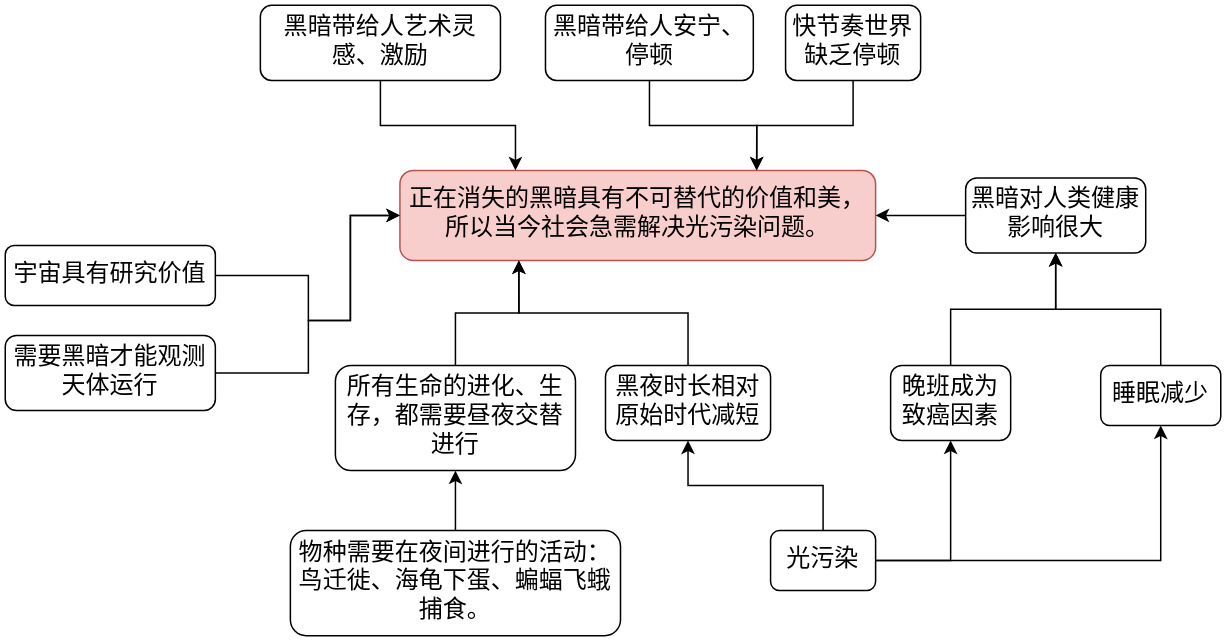
\includegraphics[width=1.0\linewidth]{批判性思维第二次作业思维图.jpg}
        \caption{思维图}
    \end{figure}

    \textbf{理由审查}:我们从思维图中对作者提出的理由进行分析,主要有一下这几个的漏洞:
    \begin{enumerate}
        \item “需要黑暗才能观测天体运行”:原文中作者提到美国的孩子大部分无法看到银河系,所以在孩子对其进行了解前,就已经由于光污染导致其无法被肉眼观测到了,
        但是在天体课上也可以对孩子进行教育,若真的对天体研究感兴趣,可以使用单孔天文望远镜,在光害相对较少的地方就能观测天体,
        使用肉眼进行天文观测已经是文艺复兴时期哥白尼的研究途径了。
        \item “所有生命的进化,都需要昼夜交替进行”:这并不完全正确,在生物进化出感光系统之前,对昼夜交替不敏感,
        当前自然界中:深海物种、大部分微生物,其进化都和昼夜无关。
        \item “晚班是光污染对人类健康影响的原因”:晚班中对人体伤害最大的应该是规律作息和过度劳累,而非光污染;
        如果将过多使用屏幕视为光污染,那么大部分工作的时间都是在受到光污染,而这并不算过度的使用照明系统。
    \end{enumerate}

    \textbf{推理关系}:作者先通过自己对黑暗的回忆,进而引出主题内容,再对当前黑暗缺乏导致的问题进行举例分析,然后提出黑暗的缺乏是由于光污染所导致的,
    最后呼吁人们节约用电减少光污染发生。从逻辑上讲,作者的推理没有很大的问题。

    \textbf{隐含假设}:本文存在的最大的一个假设就是“美国是一个发达国家,已经构建了相对发达完备的照明系统”,基于该假设才会存在光污染这类问题,
    如果考虑到还没有普及照明的平困地区,例如很多发展中国家的大部分地区,都还没有完备的照明系统,何谈光污染?所以该问题只会在社会上层建筑中才出现的,我们不能对全部地区一概而论。

    \textbf{多样性替代}:黑暗的缺少真的只是因为光污染导致的么?其实应该更多原因,当经社会的快速发展,在这个内卷时代,更少人会有闲情去欣赏星空的景色,
    思考世间万物起因,而是为了当下的琐事操心,所以黑暗的缺少也是社会快速发展的一个必然结果,
    是因为人们缺少了对自然界的好奇心,抛去了孩时的童真,从而渐渐忽视了自然界中黑暗的美。

    \textbf{总结}:基于上述分析讨论,我认为本文的逻辑思路较为清晰,从保护黑暗出发,呼吁人们对光污染问题进行重视,节约用电。
    只是作者并没有很好的将黑暗的缺乏和光污染进行区分,
    而是混为一谈,时常上文叙述光污染,下文转而对黑暗的价值进行讨论,其实二者并非充要条件,不能相互转化。

    从黑暗的角度而言,作者就事论事,从而将黑暗缺乏的直接原因归咎于光污染,但作者没有从人心和社会的角度思考这个问题,只是在浅层层面进行阐述。

    从光污染角度而言,作者也是基于自己背景的隐含假设,这是一个来自发达国家中的上层建筑问题,这并不对世界上所有地区适用,作者在写作时并没有考虑到其他发展中国家的处境。

\end{solution}

\end{document}
